\begin{wrapfigure}[18]{r}[0pt]{30mm}
	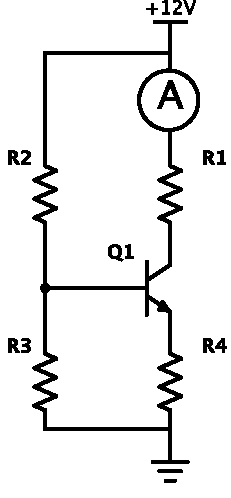
\includegraphics[width=30mm]{cc1.pdf}
	\caption{Sorgente di corrente costante.}
	\label{fig:cc1}
\end{wrapfigure}

\section{Sorgente di corrente costante}
Prima di montare il circuito riportato in Fig. \ref{fig:cc1}, abbiamo dimensionato le resistenze $R_1$ e $R_2$ del partitore in modo da avere una sorgente di corrente costante $I_L \lesssim \SI{1}{\milli\ampere}$.
Avendo scelto come $R_E=(997.3 \pm 0.2)\,\si{\ohm}$ e utilizzando la relazione $I_L+I_B=I_E \Rightarrow I_L \approx I_E$ \footnote{Nei transistor la corrente di base è almeno 100 volte inferiore rispetto a quella di collettore ed emettitore.} possiamo facilmente calcolare la tensione di base necessaria per fornire una $I_L \lesssim \SI{1}{\milli\ampere}$: $V_B=I_L \cdot R_E + 0.6V$.
Il secondo termine deriva dal fatto che tra base ed emettitore, essendo una giunzione p-n, vi è una caduta di tensione pari a $\SI{0.6}{\volt}$.

Risulta immediato impostare dunque l'equazione che permette di calcolare i valori delle resistenze nel partitore:

\begin{equation}
\frac{R_2}{R_1+R_2} V_{CC}=I_L \cdot R_E + \SI{0.6}{\volt}
\label{partitore}
\end{equation}

Evidentemente i valori delle resistenze non sono univocamente determinati da Eq. (\ref{partitore}).
Sarà dunque nostro compito scegliere una delle due in modo che non venga dissipata troppa potenza sul partitore e contemporaneamente scorra abbastanza corrente attraverso la base del transistor.
È stata scelta $R_1=99.06 \pm 0.01 \,\si{\kilo\ohm}$, valore che ci sembrava adeguato per soddisfare le due caratteristiche sopra citate.

\begin{figure}[H]
\centering
	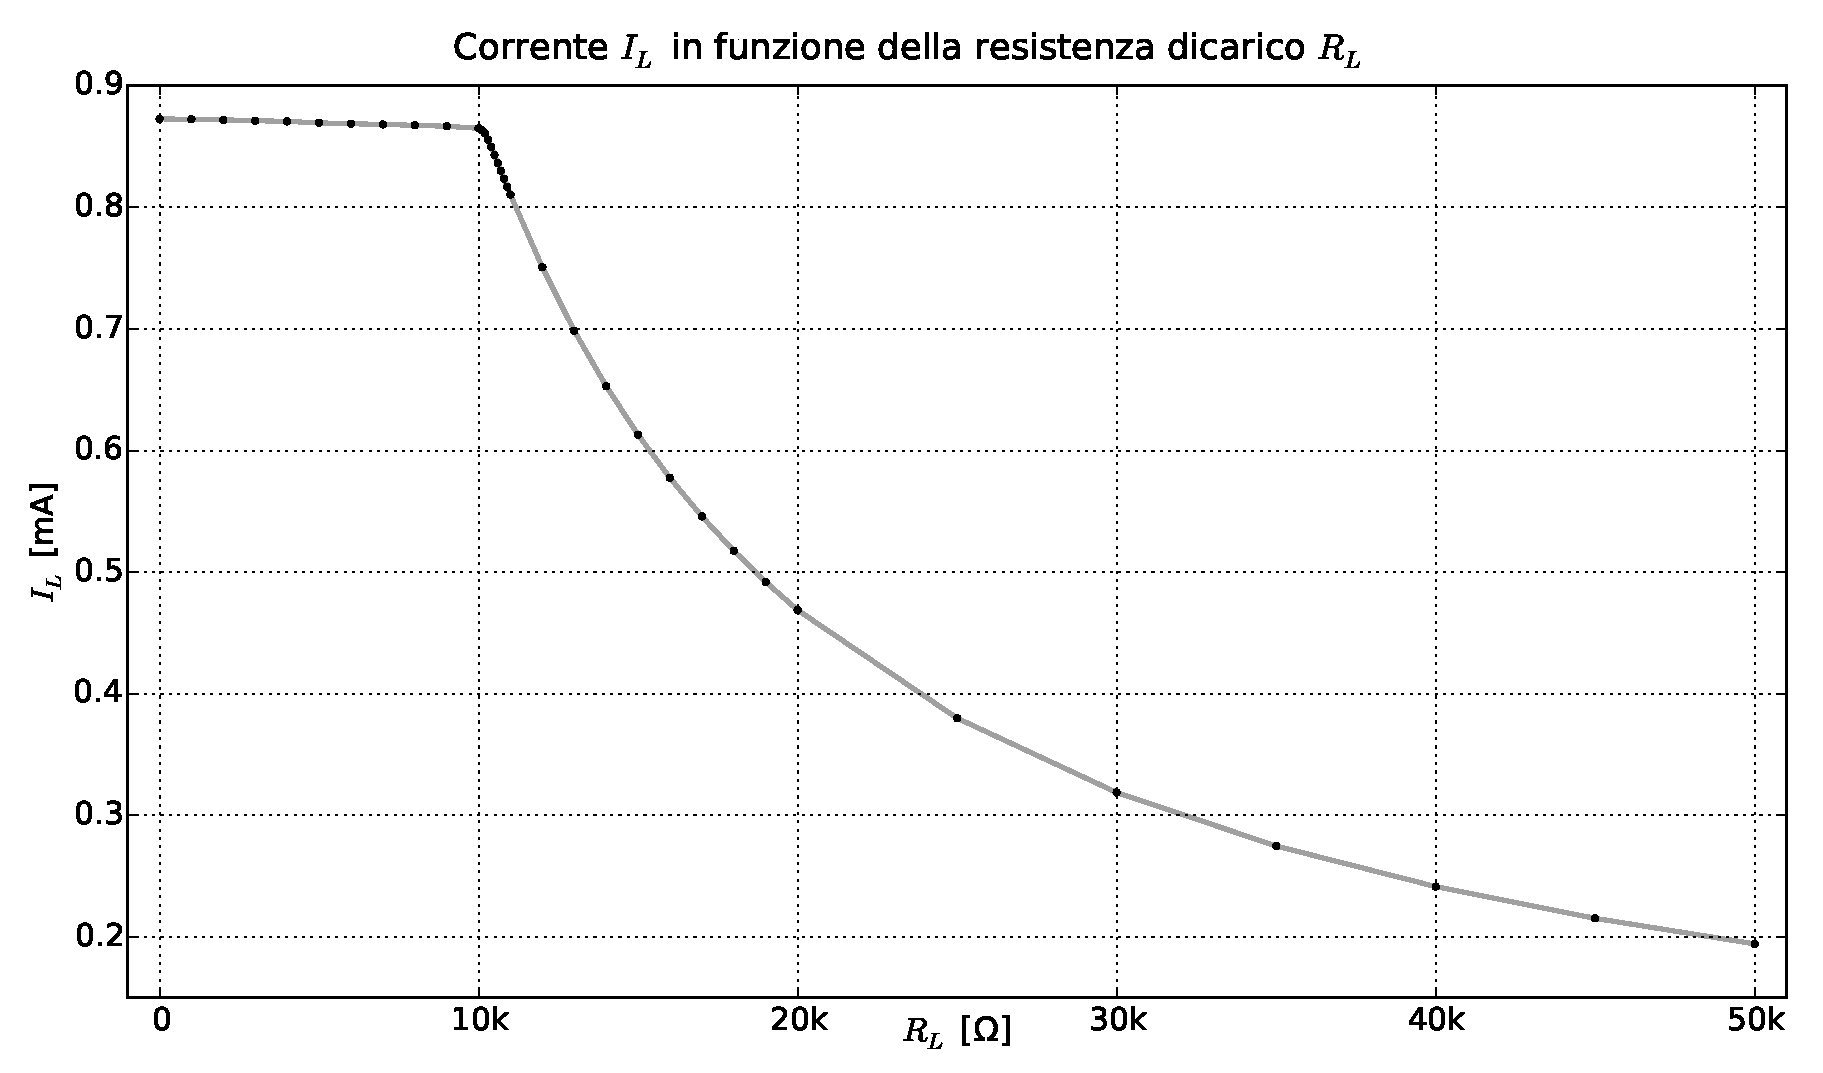
\includegraphics[scale=0.45]{sorgente.pdf}
	\caption{grafico della corrente fornita dalla sorgente di corrente in funzione del carico $R_L$. La linea in verde rappresenta il comportamento ohmico del circuito per $R_L$ elevate.}
	\label{fig:sorg}
\end{figure}

Da Eq. (\ref{partitore}) risulta $R_2 = \SI{18.6}{\kilo\ohm} $.
Il valore effettivamente utilizzato nel circuito è stato $R_2 = (18.01 \pm 0.02 )\,\si{\kilo\ohm} $.
Tale lieve discrepanza non influenzerà certamente la bontà dell'esperimento.
Infatti anche il transistor, in base alla temperatura dell'ambiente, avrà delle variazioni considerevoli delle caratteristiche intrinseche.
Ci aspettiamo dunque che il valore di corrente che successivamente andremo a misurare non avrà un valore esatto di $1\si{\milli\ampere}$. 
Il grafico di $I_L$ in funzione del carico è riportato in Fig. \ref{fig:sorg}.

Ricordiamo anzitutto che avendo avuto una $I_L<\SI{1}{\milli\ampere}$ per qualsiasi carico, abbiamo utilizzato il multimetro in modalità amperometro con un fondo-scala di $\SI{1}{\milli\ampere}$ senza mai cambiarlo (così facendo abbiamo evitato di dover correggere i dati per le diverse resistenze interne dello strumento stesso).

Come si vede graficamente, per valori di $R_L<\SI{10}{\kilo\ohm}$, la corrente di collettore è pressoché costante.
Per valori di $R_L>\SI{10}{\kilo\ohm}$ la corrente decresce.
Ciò è dovuto al fatto che, se la differenza di tensione collettore-emettitore è inferiore a \SI{0.2}{\volt}, il transistor entra in saturazione e a quel punto la corrente di  collettore non è più determinata dalla corrente di base ma dal carico $R_L$.
Risulta immediato verificare che  per un valore di carico superiore a $\SI{10}{\kilo\ohm}$ i dati obbediscono alla legge di Ohm (come si nota in Fig. \ref{fig:sorg}, linea verde).
Per ottenere una legge che fitti i dati è stato necessario correggere il circuito con la resistenza interna all'amperometro ($R_A = \SI{200}{\ohm}$).
La legge è risultata essere:
$$		I_L (R_L) =\frac{V_{cc}}{R_L+R_E+R_A}	$$